\subsection{Beispiele Elektrisches Feld}
    \subsubsection{Punktladung}
        \begin{minipage}{0.41\linewidth}
            \begin{footnotesize}
                \begin{center}
                    \vspace{2mm}
                    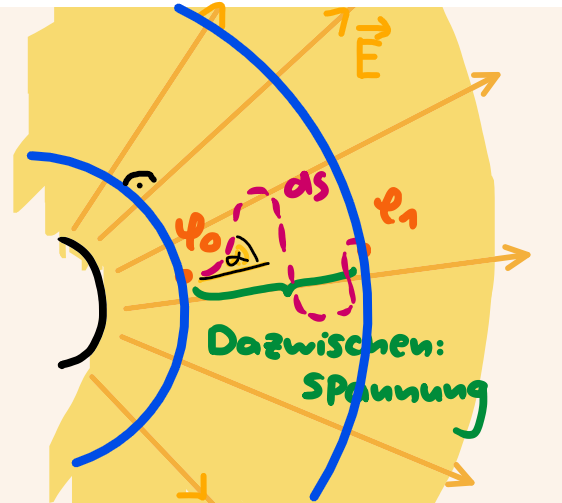
\includegraphics[width = 25mm]{src/images/inhom_potentialfeld.png}
                \end{center}
            \end{footnotesize}
        \end{minipage}
        \begin{minipage}{0.58\linewidth}
            \begin{scriptsize}
                \begin{center}
                    \begin{empheq}[box = \fbox]{align*}
                    %\mathbox{
                        U &= \int_{1}^{2}E\cdot\cos (\alpha) ds\\
                        &= \int_{1}^{2}\vec{E}(r)\:\vec{dr}
                    \end{empheq}
                    Auf \colorbox{Cyan}{Kreis $\Phi_{0/1}$} stets selbes Potential/Spannung
                \end{center}
            \end{scriptsize}
        \end{minipage}

    \subsubsection{Spannungswaage / Thompson-Waage}
        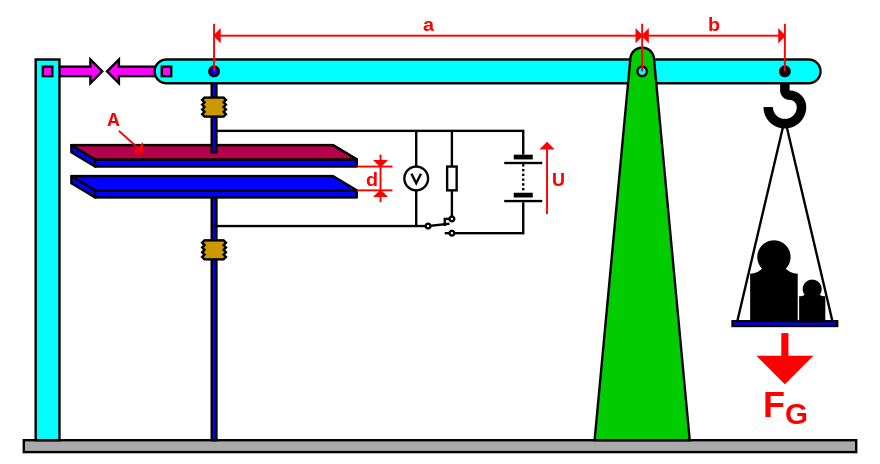
\includegraphics[width = 0.99\linewidth]{src/images/spannungswaage.png}
        \begin{minipage}{0.63\linewidth}
            \centering
            Kräftegleichgewicht:
            \begin{empheq}[box = \fbox]{align*}
                F_E &= \frac{E \cdot Q}{2} = \frac{1}{2} \varepsilon_0 \varepsilon_r \frac{A}{d^2} U^2\\
                F_G &= m \cdot g\\
                a \cdot F_E &= b \cdot F_G
            \end{empheq}
        \end{minipage}
        \begin{minipage}{0.35\linewidth}
            \begin{scriptsize}
                \begin{empheq}{align*}
                    F_E &= \text{elektrostatische Kraft}\\
                    F_G &= \text{Gewichtskraft}\\
                    m &= \text{Masse} [kg]\\
                    g &= \text{Fallbeschleunigung}\\
                    E &= \text{Elektrische Feldstärke}\\
                    Q &= \text{Ladungsmenge}\\
                    \varepsilon_r &= \text{Permittivität}
                \end{empheq}
            \end{scriptsize}
        \end{minipage}


    \subsubsection{Elektrisches Feld Kugel / Punktladung}
        \begin{minipage}{0.59\linewidth}
            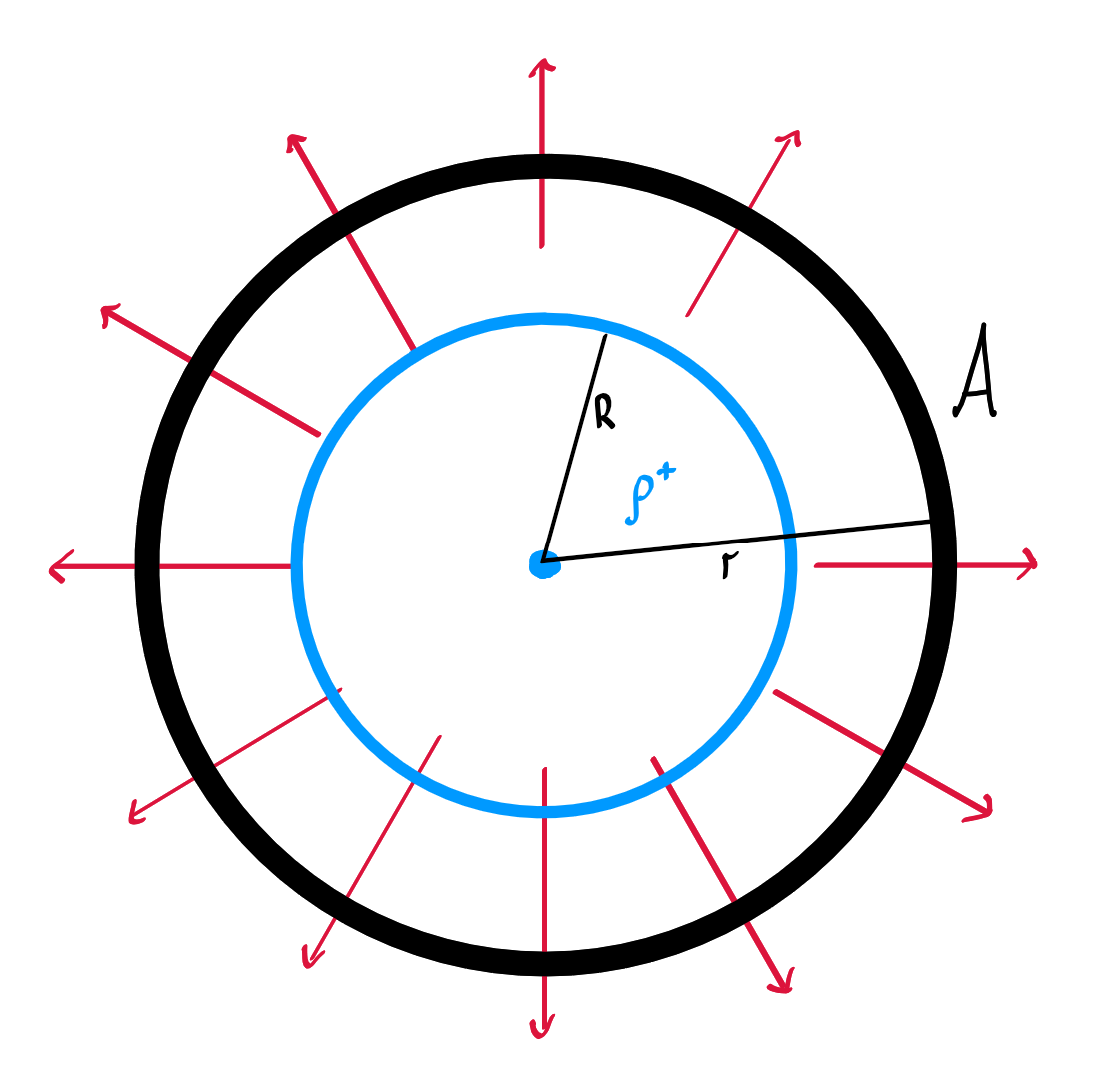
\includegraphics[width = \linewidth]{src/images/e-feld_punktladung.png}
        \end{minipage}
        \begin{minipage}{0.39\linewidth}
            \begin{empheq}{align*}
                \oint \vec{E} \vec{dA} &= \frac{1}{\varepsilon_0} \int \rho dV\\
                \rho&= \frac{Q}{V} = \frac{3Q}{4 \pi R^3}
            \end{empheq}
        \end{minipage}
        \[\begin{array}{c | c}
            r < R & r \geq R\\
            \hline \hline
            \Rightarrow E \cdot 4 \pi r^2 = \frac{\rho \cdot \frac{4}{3} \pi r^3}{\varepsilon_0} & \Rightarrow E \cdot 4 \pi r^2 = \frac{\rho \cdot \frac{4}{3}\pi R^3}{\varepsilon_0}\\
            \Rightarrow E = \frac{\rho r}{3 \varepsilon_0} = \frac{1}{4 \varepsilon_0 \pi } \frac{Q r}{R^3} & \Rightarrow E = \frac{\rho R^3}{3 \varepsilon_0 r^2} = \frac{1}{4 \varepsilon_0 \pi} \frac{Q}{r^2}
        \end{array}\]

    \vfill \null \columnbreak

    \subsubsection{Elektrisches Feld gerader Leiter}
        \begin{minipage}{0.39\linewidth}
            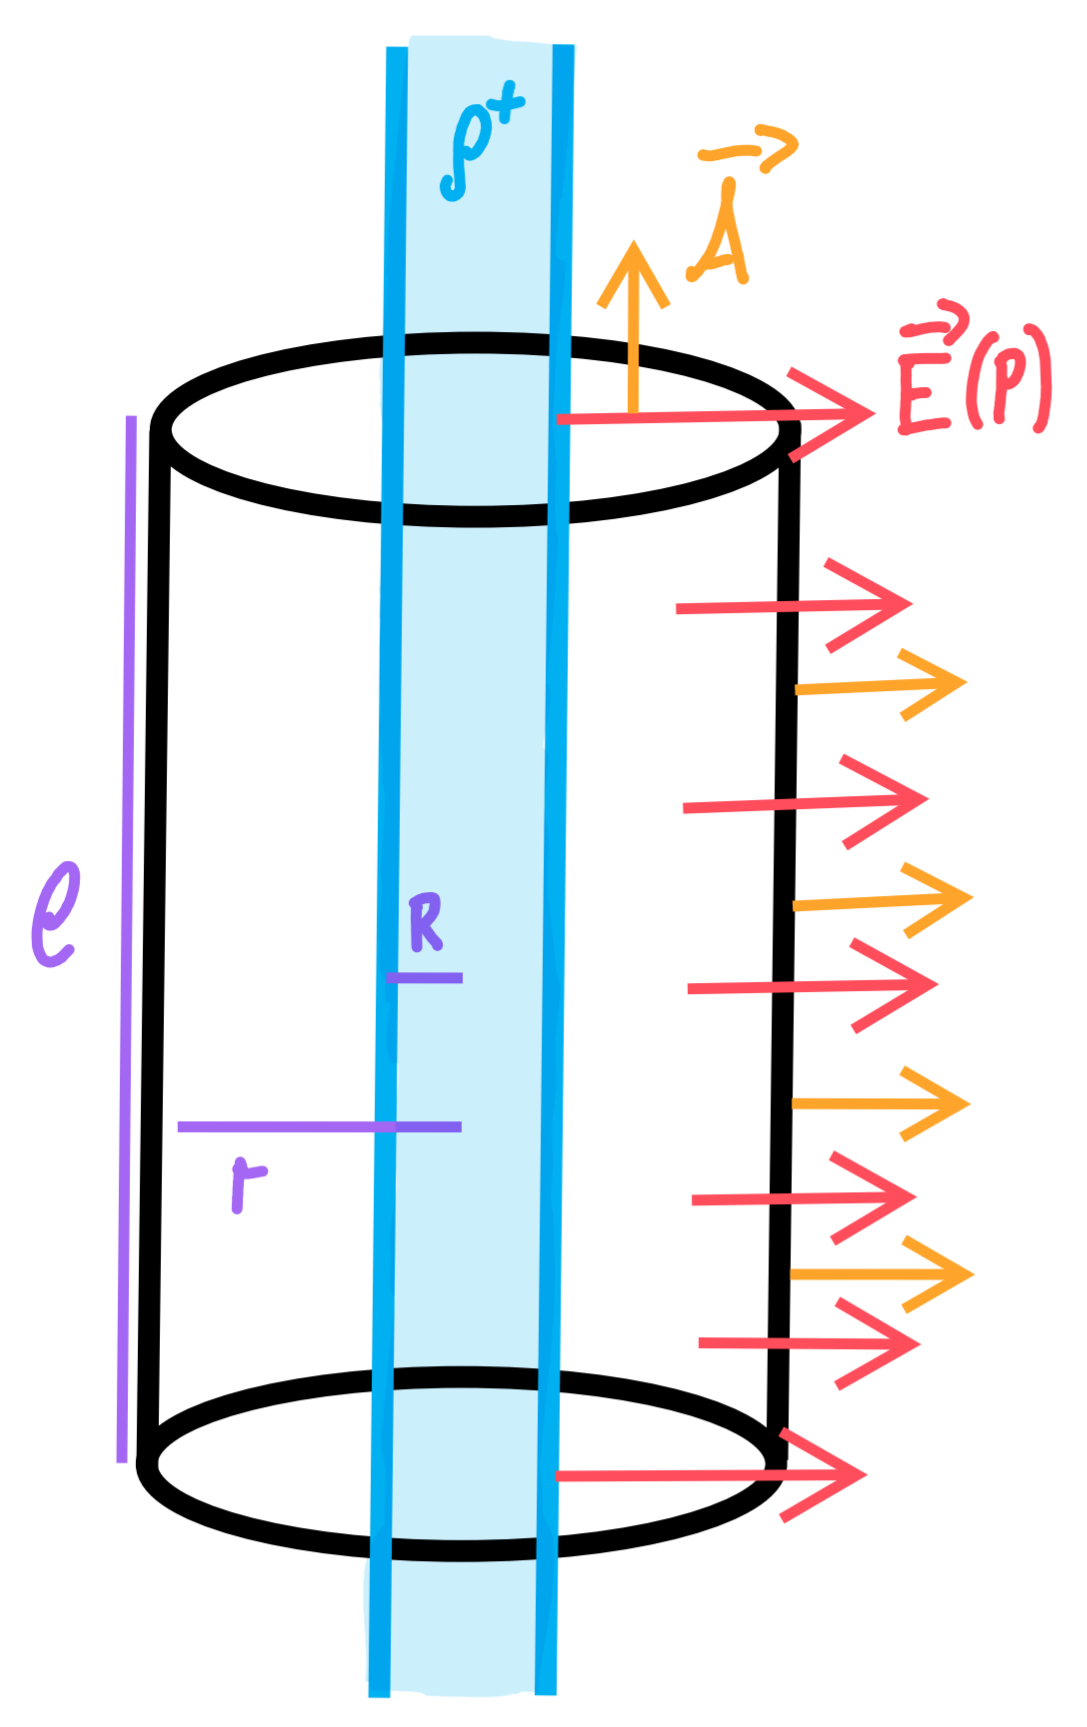
\includegraphics[width = \linewidth]{src/images/e-feld_gerader_leiter.png}
        \end{minipage}
        \begin{minipage}{0.59\linewidth}
            \begin{empheq}{align*}
                \oint \vec{E} \vec{dA} &= \frac{1}{\varepsilon_0} \int \rho dV\\
                \rho &= \frac{Q}{V} = \frac{3Q}{4 \pi R^3}\\
            \end{empheq}
        \end{minipage}
        \[\begin{array}{c | c}
            r < R & r \geq R\\
            \hline \hline
            E \cdot 2 \pi r \cdot l = \frac{\rho}{\varepsilon_0} \pi r^2 l & E \cdot 2 \pi r \cdot l = \frac{\rho}{\varepsilon_0} \pi R^2 l\\
            E = \frac{\rho}{2 \varepsilon_0} r & E = \frac{\rho}{2 \varepsilon_0} \frac{R^2}{r}
        \end{array}\]

    \subsubsection{Elektrisches Feld Platte}
        \begin{minipage}{0.49\linewidth}
            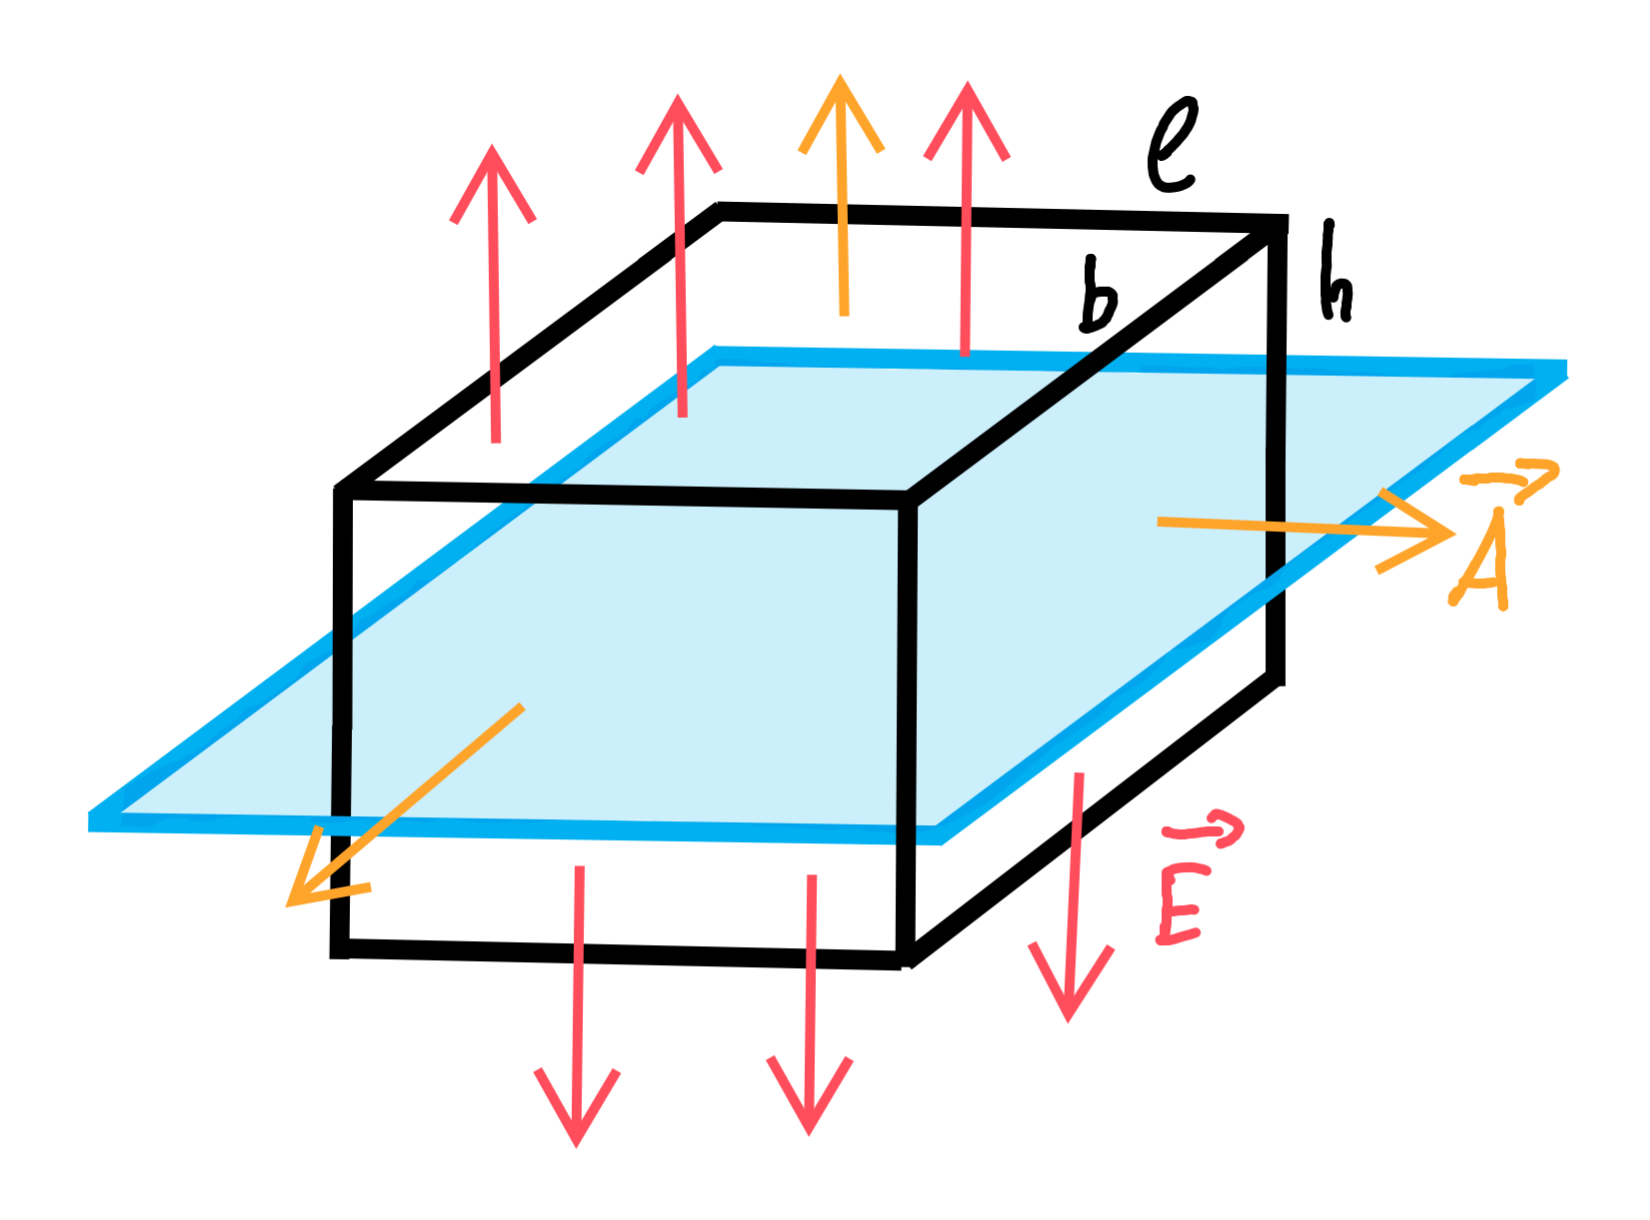
\includegraphics[width = \linewidth]{src/images/e-feld_platte.png}
        \end{minipage}
        \begin{minipage}{0.49\linewidth}
            \begin{empheq}{align*}
                &\oint \vec{E} \vec{dA} = \frac{1}{\varepsilon_0} \int \rho dV\\
                &\rho = \frac{Q}{A} = \frac{Q}{l \cdot b}\\
                \Rightarrow &E \cdot 2 l \cdot b = \frac{1}{\varepsilon_0} l \cdot \rho\\
                \Aboxed{\Rightarrow &E = \frac{\rho}{2 \varepsilon_0}}
            \end{empheq}
        \end{minipage}

    \subsubsection{Arten von Kondensatoren}
        {\centering \underline{\textbf{Plattenkondensator}} \par}
        \begin{minipage}{0.49\linewidth}
            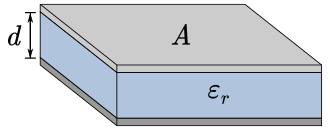
\includegraphics[width = \linewidth]{src/images/plattenkond.png}
        \end{minipage}
        \begin{minipage}{0.49\linewidth}
            \begin{empheq}[box=\fbox]{align*}
                C &= \varepsilon_0 \cdot \varepsilon_r \frac{A}{d}
            \end{empheq}
        \end{minipage}
        
        {\centering \underline{\textbf{Zylinderkondensator}} \par}
        \begin{minipage}{0.49\linewidth}
            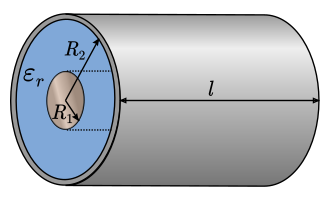
\includegraphics[width = \linewidth]{src/images/zylinderkond.png}
        \end{minipage}
        \begin{minipage}{0.49\linewidth}
            \begin{empheq}[box=\fbox]{align*}
                C &= 2\pi \varepsilon_0\cdot \varepsilon_r \frac{l}{\ln(\frac{r_2}{r_1})}
            \end{empheq}
        \end{minipage}
        
        {\centering \underline{\textbf{Kugelkondensator}} \par}
            \begin{minipage}{0.39\linewidth}
                {\centering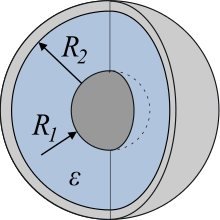
\includegraphics[width = 0.9\linewidth]{src/images/kugelkondensator.png} \par}
            \end{minipage}
            \begin{minipage}{0.59\linewidth}
                \begin{empheq}[box=\fbox]{align*}
                    C &= 4 \pi \varepsilon_0 \cdot \varepsilon_r \left(\frac{r_1 \cdot r_2}{r_2 - r_1}\right)
                \end{empheq}
            \end{minipage}